

%%%%%%%%%%%%%%%%%%%%
% PLOT: FIELD CT   %
%%%%%%%%%%%%%%%%%%%%
\begin{SCfigure}[1.][tb]
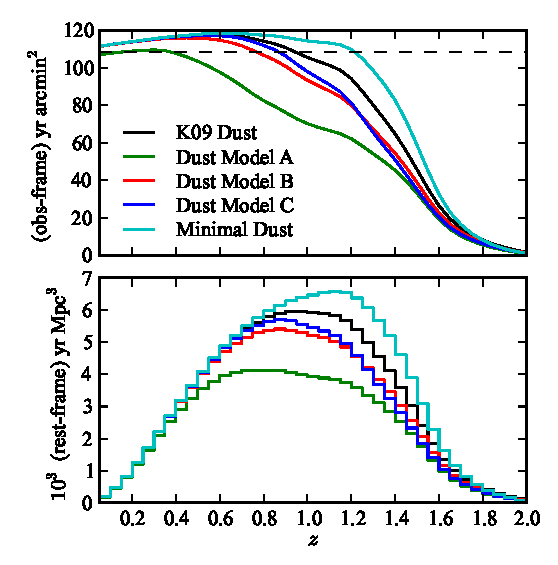
\includegraphics[width=0.6\textwidth]{figures/fieldrate/ctarea1.eps}
\caption[Effective visibility time as a function of redshift]{\emph{Top panel:} 
The observer-frame effective visibility time multiplied by observed
area, as a function of supernova redshift. The horizontal dotted line
shows the area of the ACS field multiplied by the time spanned by the
observations in each cluster.  \emph{Bottom panel:} The rest-frame
volume-time searched in each redshift bin of $\Delta z = 0.05$. In
each panel, the black line shows our main result for the effective
visibility time, based on simulations using the K09 dust
distribution. The green, red, blue and cyan lines show the results for
alternative dust distributions.\label{fig:ctarea1}}
\end{SCfigure}

Figure~\ref{fig:ctarea1} (top panel, black line) shows the
observer-frame effective visibility time times area ($T(z) \Theta$
from Eq.~\ref{eq:fieldrate}) as a function of SN redshift. For
reference, the horizontal dotted line shows an approximate calculation
of this value, multiplying the area of the ACS field
(11.65~arcmin$^2$) by the time difference between 10~days before the
first observation and 10~days after the last observation. In reality
the area actually observed is slightly more complicated and SNe are
detected over a slightly larger time range. From $z=0$, the effective
visibility time actually increases slightly out to $z \sim 0.5$ as SN
light curves are time-dilated and are thus visible for
longer. Afterwards, we begin to miss SNe that peak during the
observations. In the lower panel of Figure~\ref{fig:ctarea1}, we convert
to the rest-frame time-volume observed in each redshift bin of $\Delta
z = 0.05$ (Fig.~\ref{fig:ctarea1}, lower panel) using the assumed
cosmology.  The denominator of Equation~(\ref{eq:fieldrate}) is
obtained by summing over the redshift bin of
interest. Table~\ref{tab:results} shows the results, in bins of
$\Delta z = 0.4$ and also in bins of $\Delta z = 0.5$. We now discuss
the systematic uncertainties
associated with lensing, SN type determination, host-galaxy dust, and
variations in SN properties.


\subsection{Type Determination} \label{sec:systyping}

Only four of our SN candidates have spectroscopically confirmed
types -- for the remaining candidates there is some uncertainty in
type. It is difficult to precisely quantify the uncertainty in our
heterogeneous typing method, mainly because the information
used to type each SN varies widely. In practice
however, the uncertainty is quite small. Consider the candidates
designated as SN~Ia: all three SNe~Ia at $z<0.9$ are spectroscopically
confirmed. At $z \gtrsim 0.9$, any SN bright enough to be detected is
overwhelmingly likely to be Type~Ia due to the faintness of
core-collapse SNe relative to SNe~Ia \citep[see, e.g.,][Meyers et al.,
submitted]{dahlen04a,li10a}. Furthermore, while ``probable''
candidates are not as certain as ``secure'' candidates, this is still
a fairly high-confidence type determination: A ``probable'' SN~Ia
means that a SN~Ia light curve template has a $\chi^2$ $P$-value that
is $10^3$ times larger than any SN~CC value. A Bayesian analysis would
therefore yield a type uncertainty close to zero for such candidates,
regardless of the prior used.


%%%%%%%%%%%%%%%%%%%%%%
% TABLE: FIELD RATES %
%%%%%%%%%%%%%%%%%%%%%%
\begin{table}
\caption{\label{tab:results}Results: field SN~Ia rate}
\begin{center}
\begin{footnotesizetabular}{lcccccc}
\hline
\hline
Redshift bin & $\bar{z}$ & $N_{\rm SN~Ia}$ & Denom & Rate & (stat) & (sys) \\
\hline
$0.2 < z \le 0.6$ & 0.442  & $0.00^{+0.00}_{-0.00}$ &2.332 & 0.00  & $^{+0.50}_{-0.00}$ & $^{+0.00}_{-0.00}$ \\
$0.6 < z \le 1.0$ & 0.807  & $5.25^{+0.25}_{-1.25}$ &4.464 & 1.18  & $^{+0.60}_{-0.45}$ & $^{+0.11}_{-0.28}$ \\
$1.0 < z \le 1.4$ & 1.187  & $5.63^{+0.63}_{-0.63}$ &4.243 & 1.33  & $^{+0.65}_{-0.49}$ & $^{+0.30}_{-0.26}$ \\
$1.4 < z \le 1.8$ & 1.535  & $1.12^{+0.12}_{-1.12}$ &1.453 & 0.77  & $^{+1.07}_{-0.54}$ & $^{+0.34}_{-0.77}$ \\
\\
\hline
\\
$0.0 < z \le 0.5$ & 0.357  & $0.00^{+0.00}_{-0.00}$ &1.624 & 0.00  & $^{+0.71}_{-0.00}$ & $^{+0.00}_{-0.00}$ \\
$0.5 < z \le 1.0$ & 0.766  & $5.25^{+0.25}_{-1.25}$ &5.321 & 0.99  & $^{+0.51}_{-0.38}$ & $^{+0.08}_{-0.24}$ \\
$1.0 < z \le 1.5$ & 1.222  & $6.75^{+0.75}_{-1.75}$ &4.906 & 1.38  & $^{+0.61}_{-0.47}$ & $^{+0.33}_{-0.43}$ \\
$1.5 < z \le 2.0$ & 1.639  & $0.00^{+0.00}_{-0.00}$ &0.890 & 0.00  & $^{+1.30}_{-0.00}$ & $^{+0.00}_{-0.00}$ \\
\hline
\end{footnotesizetabular}

\end{center}
{\footnotesize {\bf Note.} --- ``Denom'' is the denominator of
equation \ref{eq:fieldrate} (total rest frame time-volume searched in
this bin) and has units $10^4$ yr Mpc$^3$. The rate is given in units
$10^{-4}$ yr$^{-1}$ Mpc$^{-3}$. $N_{\rm SN~Ia}$ is the observed number
of SNe in the bin, with the uncertainty due to type determination. The
non-integer number of SNe in each bin is attributable to the two
candidates without spectroscopic redshifts. These candidates are
assigned redshift ranges that are spread over multiple bins.}
\end{table}

The ``plausible'' candidates are perhaps the only candidates with
significant type uncertainty. We quantify this uncertainty in a manner
similar to \citet{dahlen08a}: The lower limit on the number of SNe~Ia
discovered is given by assuming that all ``plausible'' SNe~Ia are in
fact SNe~CC, and the upper limit is given by assuming that all
``plausible'' SNe~CC are in fact SNe~Ia.  These limits are shown as
uncertainties in $N_{\rm SN~Ia}$ in Table~\ref{tab:results} and
those uncertainties are included in the systematic error.

%Still, we quantify the typing systematic error by assigning an
%asymmetric error of 0.25 SNe for ``probable'' confidence SNe and 0.5
%for ``plausible'' confidence SNe. That is, ``probable'' SNe~Ia are
%counted at $1^{+0}_{-0.25}$ SNe~Ia, ``plausible'' SNe~Ia are counted
%as $1^{+0}_{-0.5}$ SNe~Ia, ``probable'' SNe~CC are counted as
%$0^{+0.25}_{-0}$ SNe~Ia, and ``plausible'' SNe~CC are counted as
%$0^{+0.5}_{-0}$ SNe~Ia.

For the two candidates without spectroscopic host redshifts, we assign
a redshift range consistent with the SN light curve and/or host galaxy
photometry, as follows: For SCP06E12, we use the range $0.8<z<1.2$. As
there is uncertainty about both the type and cluster membership, we
count SCP06E12 as $0.5 \pm 0.5$ field SNe~Ia. The situation is similar
for SCP06N32: the light curve is consistent with an SN~Ibc at $z \sim
0.9$, but also with an SN~Ia at $z \sim 1.3$. We therefore assign a
redshift range of $1.1 < z < 1.5$ and count it as $0.5 \pm 0.5$ field
SNe~Ia. Finally, note that the spectroscopic host galaxy redshift of
$z=1.44$ for SCP06X26 is tentative because it is based on a single
(low signal-to-noise) emission line. This redshift uncertainty
contributed to the low-confidence ``plausible'' in the type and the
typing systematic error encompasses the possibility that SCP06X26 is
not an SN~Ia at this redshift. This makes the rate for the highest
redshift bin $1.4 < z <1.8$ an upper limit only. However, note that
the light curve of SCP06X26 is completely consistent with a typical
$z=1.44$ SN~Ia.


\subsection{Lensing Due to Clusters} \label{sec:lensing}

The presence of a massive galaxy cluster in each of the 25 observed
fields presents a complication for measuring the volumetric field
rate. A cluster will preferentially magnify sources behind it
(increasing the discovery efficiency of SNe), and will also shrink the
source plane area $\Theta$ behind the cluster (decreasing the number
of SNe discovered) \citep[e.g.,][]{goobar09a}. Fortunately the effect
on the calculated rates in this survey is small, for two
reasons. First, the high redshifts of the clusters means that the
volume of interest in the cluster backgrounds is close to the clusters
and therefore not lensed very efficiently. Second, the two effects
(magnification and source plane area shrinkage) are opposing in terms
of number of SNe discovered.  Furthermore, we have already excluded
from the analysis the central $20''$ of each field, where lensing
effects are the largest.

We have calculated the magnitude of each lensing effect on the
remaining outer regions using a simple lensing model: We assume each
cluster has a mass of $M_{200} = 4\times 10^{14}~M_\odot$ (the
approximate average mass in our sample, as reported by Jee et al., in
preparation) and an NFW mass profile. We distribute clusters according
to their redshifts and calculate the lensing effect on the 25 annular
regions $20'' < r < 100''$ around the clusters. The distribution of
magnification in these regions as a function of source redshift is
shown in Figure~\ref{fig:magpdf}. The magnification is quite small:
even at a source redshift of $z=1.8$, most of the area is magnified by
less than 10\%. As a rough estimate of the effect on the derived
rates, we show the average magnification for each source redshift, and
the effect such a magnification would have on the effective visibility
time at this redshift. The effect is only a few percent at $z \lesssim
1.4$ but starts to increase steeply towards $z=1.8$. In
Figure~\ref{fig:sourcearea} we show the decrease in the source area as
a function of redshift, which translates directly into a decrease in
the effective visibility time $\times$ area. The decrease is close to
linear with redshift past $z=1.2$, reaching $\sim$13\% at $z=1.8$.


%%%%%%%%%%%%%%%%%%%%%%%%%%%%%%%%%%%%%
% Figure: Lensing Magnification PDF %
%%%%%%%%%%%%%%%%%%%%%%%%%%%%%%%%%%%%%
\begin{SCfigure}[1.][tb]
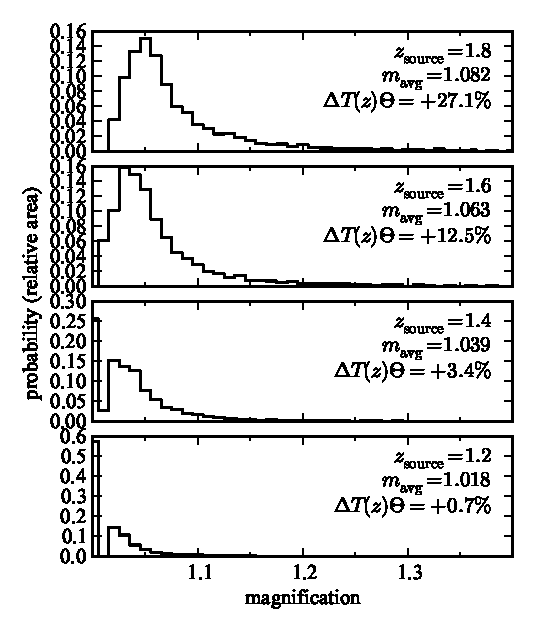
\includegraphics[width=0.6\textwidth]{figures/fieldrate/magpdf.eps}
\caption[Lensing magnification distribution in lensing simulation]
{Lensing magnification distribution in our lensing simulation, as a
function of source redshift. The distribution is taken from the
regions at radius $20'' < r < 100''$ in each of 25 cluster fields (the
approximate extent of the regions used in the rate analysis). For each
source redshift, the average magnification $m_{\rm avg}$ is given. If
all simulated SNe at this redshift were magnified by $m_{\rm avg}$,
the effective visibility time would increase by $\Delta
T(z) \Theta$. At $z<1.4$ lensing magnification has only a $\lesssim
3\%$ effect on the detectability of SNe.\label{fig:magpdf}}
\end{SCfigure}


%%%%%%%%%%%%%%%%%%%%%%%%%%%%%%%%%%%%%%%%%%
% Figure: Lensing Source area distortion %
%%%%%%%%%%%%%%%%%%%%%%%%%%%%%%%%%%%%%%%%%%
\begin{SCfigure}[1.][tb]
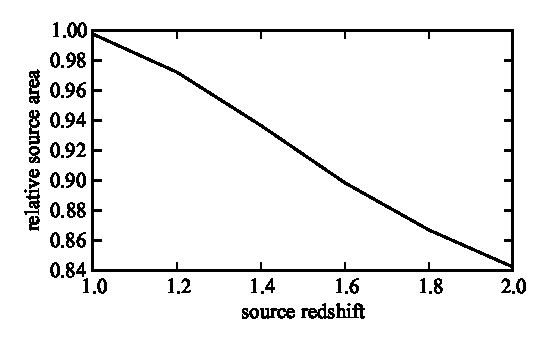
\includegraphics[width=0.6\textwidth]{figures/fieldrate/sourcearea.eps}
\caption[Source-plane area versus observed area in lensing
  simulation]{True source-plane area relative to the observed area in
  our lensing simulation, as a function of source redshift. The
  relative area is for regions at radius $20'' < r < 100''$ in each of
  the 25 cluster fields (the approximate extent of the regions used in
  the analysis). \label{fig:sourcearea}}
\end{SCfigure}


We conclude from these simulations that the two effects cancel to
within a few percent of the total rate, over the redshift range of
interest: At $z=1.4$, magnification increases SN detectability by
$\sim$3\% and source-area reduction decreases detectability by
$\sim$6\%. At $z=1.6$, the increase is $\sim$12\%, and the decrease is
$\sim$10\%. At $z=1.8$ the increase overwhelms the decrease
($\sim$27\% versus $\sim$13\%), but there will be very few SNe
detected beyond $z \sim 1.6$ (see Fig.~\ref{fig:ctarea1}). Therefore,
we have not made an adjustment for these effects. Furthermore, the
size of each effect is much smaller than other sources of systematic
error considered below. For example, the average magnification at
$z=1.8$ is only $\sim$1.08 ($-0.08$~mag), whereas below we consider
the effect of changing the luminosity of all SNe in our simulation by
$\pm 0.2$~magnitudes. As a result, we do not assign a specific
systematic error to the lensing effects.


%%%%%%%%%%%%%%%%%%%%%%%%%%%%%%%%%%%%%%%%%%%%%%%%%%%%%%%%%%%%%%%%%%%%%%%%%%%%%
%                        PLOT: DUST EXTINCTION PDF                          %
%%%%%%%%%%%%%%%%%%%%%%%%%%%%%%%%%%%%%%%%%%%%%%%%%%%%%%%%%%%%%%%%%%%%%%%%%%%%%
\begin{SCfigure}[1.][bt]
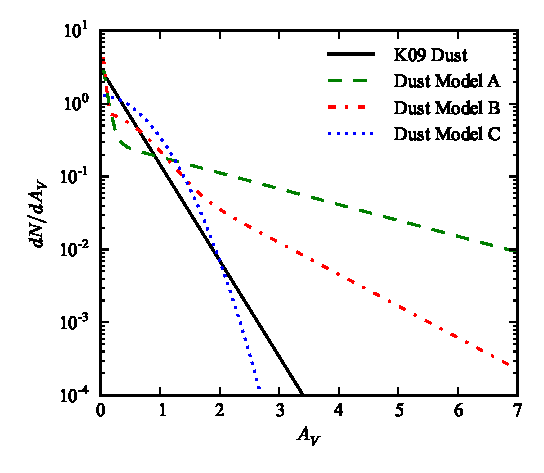
\includegraphics[width=0.6\textwidth]{figures/fieldrate/extinctiondist.eps}
\caption[Dust extinction distributions used in field rate
  calculation]{Host galaxy dust extinction distributions. The K09
  distribution is used for our main result. Models A, B, and C are
  similar to the models of the same name examined in \citet{dahlen08a}
  and are based on results from \citet{hatano98a}, \citet{riello05a}
  and \citet{neill06a}, respectively. These alternative distributions
  are used here to investigate possible systematic error due to host
  galaxy dust.\label{fig:extinction}}
\end{SCfigure}


%%%%%%%%%%%%%%%%%%%%%
% PLOT: FIELD RATES %
%%%%%%%%%%%%%%%%%%%%%
\begin{figure}
\begin{center}
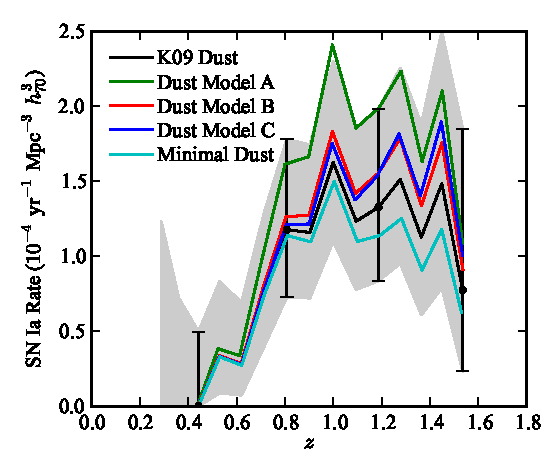
\includegraphics[width=0.5\textwidth]{figures/fieldrate/fieldrates1.eps}%
\includegraphics[width=0.5\textwidth]{figures/fieldrate/fieldrates2.eps}
\end{center}
\caption[Volumetric SN Ia rate results with systematic 
uncertainties]{The volumetric SN Ia rate in four redshift bins (points
with error bars) of width $\Delta z = 0.4$. The error bars represent
the statistical-only error. The black line shows the rate calculated
in a moving bin of width $\Delta z = 0.4$ (grey regions represent
uncertainty). Note that the points with error bars are uncorrelated
errors (using non-overlapping bins), while the uncertainty in the
moving bin is correlated from point to point.
\emph{Left Panel}: The green, red, blue and cyan lines show the 
rate (with no uncertainty) assuming alternative SN color distributions.
\emph{Right Panel}: The red and blue lines show the rate assuming 
that all SNe are brighter or dimmer by $\pm 0.2$~mag.
\label{fig:fieldrates1}}
\end{figure}

\subsection{Dust Extinction} \label{sec:sysdust}

The degree to which SNe are affected by host galaxy dust extinction is
perhaps the largest systematic uncertainty in SN~Ia rate studies. To
evaluate the effect on the derived rates, we consider four alternative
extinction distributions. Three of these are comparable to
distributions examined in \citet{dahlen08a}. The first, labeled
``Model A,'' is used in their main result and is based
on \citet{hatano98a}. We approximate this distribution as
\begin{equation}
P(A_V) = \frac{0.61}{2}e^{-A_V/2} + \frac{0.39}{0.07}e^{-A_V/0.07}.
\end{equation}
The second, labeled ``Model B,'' is based
on \citet{riello05a} and is approximated here by
\begin{equation}
P(A_V) = 0.35 \delta(A_V) + 
\frac{0.40 \times 2}{0.6 \sqrt{2\pi}}e^{-A_V^2/(2 \times 0.6^2)} + 0.25 e^{-A_V}.
\end{equation}
The third, labeled ``Model C,'' is based on \citet{neill06a} and is given by
\begin{equation}
P(A_V) = \frac{2}{0.62 \sqrt{2\pi}}e^{-A_V^2/(2 \times 0.62^2)}.
\end{equation}
These distributions are reproduced in Figure~\ref{fig:extinction}, and
the corresponding distributions of SN color are shown in
Figure~\ref{fig:dists_field} (right panel).  In addition to these three
distributions, we also consider a distribution with minimal dust,
where we assume the SNLS $z<0.6$ sample is complete and fit it
with a skewed Gaussian distribution.  The effective visibility time
for each dust model is shown in Figure~\ref{fig:ctarea1} and the
corresponding SN rate results are shown in
Figure~\ref{fig:fieldrates1} (left panel).

Of all the models, Model A produces the most strikingly different
results for the effective visibility time. Even in the lowest redshift
bin ($0.2<z<0.6$) it implies that 10\% of SNe are missed due to dust,
relative to the K09 model. In the $0.6<z<1.0$ redshift bin, it yields
effective visibility times lower by 27\%, while Models B, C and the
minimal dust model result in changes of only $-7\%$, $-3\%$, and
$+3\%$ respectively. This is unsurprising: In dust model A, 26\% of
SNe have host galaxy extinctions $A_V > 2$ while this fraction is
$<4\%$ in model B and $<1\%$ in models K09 and C. In the $1.0 < z <
1.4$ bin model A has the largest effect: $-33\%$ compared to the K09
model.

For the systematic error associated with the choice of dust model we
take the minimal dust model as the extreme lower limit and model B/C
as the upper limit, regarding model A as an outlying model. This
systematic error is propagated and included in
Table~\ref{tab:results}.

\subsection{Other SN Properties}

Other assumptions about SN properties (besides dust extinction) can
affect the results. To first order, changing the assumed distributions
of $s$ or changing the assumed spectral time series will affect the
detection efficiency by increasing or decreasing the luminosity of the
simulated SN. To jointly capture these effects, we shift the absolute
magnitude of the simulated SNe~Ia by $^{+0.2}_{-0.2}$~mag and
recalculate the control times. To first order, this is equivalent to
shifting the $s$ distribution by $\Delta s = 0.2/\alpha \sim 0.16$ (or
shifting the $c$ distribution by $\Delta c = 0.2/\beta \sim
0.09$). The effect on the results is shown in
Figure~\ref{fig:fieldrates1} (right panel) and this range of
uncertainty is included in the systematic error in
Table~\ref{tab:results}.

\vspace{0.4in}
